De NAND\index{NAND} geeft een negatief resultaat als beide ingangen 1 zijn, de uitgang is dan 0.

\rowcolors{2}{gray!10}{gray!20}
\begin{tabular}{ |c|c|c| }
\hline
\rowcolor{gray!60}
	Input 1 & Input 2 & Output \\
	\hline
	0 & 0 & 1 \\
	\hline
	0 & 1 & 1 \\
	\hline
	1 & 0 & 1 \\
	\hline
	1 & 1 & 0 \\
	\hline
\end{tabular}

Het symbool voor de NAND is weergegeven in figuur \ref{symbool:nand}

\begin{figure}[h]
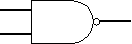
\includegraphics{nand_symbool}
\centering
\caption{Symbool van een NAND}
\label{symbool:nand}
\end{figure}

De NAND wordt gebouwd door gebruik te maken van twee transistoren waarvan de beide basis de ingang vormen en een weerstand (figuur \ref{circuit:nand}.

\begin{figure}[h]
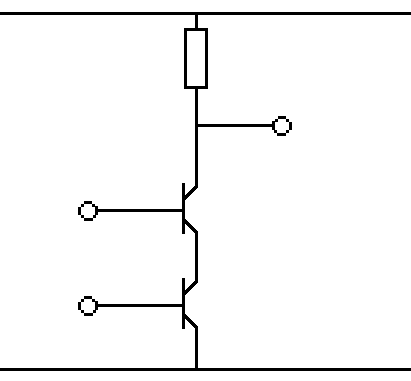
\includegraphics{nand_circuit}
\centering
\caption{NAND circuit}
\label{circuit:nand}
\end{figure}

De NAND-technologie kan je tegen komen in flash memory.

